\chapter{Inleiding}
De Esenthel editor bevat een tool om je 3D wereld vorm te geven. Tutorials over het gebruik daarvan vind je op de Esenthel website. In dit deel leer je hoe je die wereld gebruikt in je programma.

\section{De wereld laden}
Meestal gebeurt het laden en updaten van een 3D wereld in een afzonderlijke gamestate. Bij de start van een programma wil je waarschijnlijk eerst enkele menu's en misschien een game lobby tonen. Pas daarna schakel je over naar een gamestate die je wereld toont. Om de code in dit deel eenvoudig te houden, slaan we die stappen over en werken we enkel met een 3D wereld in de standaard gamestate. Daarin zijn 4 functies belangrijk:

\begin{itemize}
	\item de Init functie,
	\item de Update functie,
	\item de Draw functie en
	\item de Render functie.
\end{itemize}

\subsection{Init}
In tegenstelling tot een 2D wereld, heeft een 3D wereld enkele standaard vereisten: Physics, een wereld en een camera. (In principe kan het ook zonder de wereld, maar dat is een heel ander soort game.) Deze drie worden ge\"initialiseerd in de Init functie:

\begin{code}
// enable physics engine
Physics.create(EE_PHYSX_DLL_PATH);
   
// load game world
Game.World.activeRange(D.viewRange());
Game.World.New(=== insert world here ===);
if (Game.World.settings().environment) {
  Game.World.settings().environment->set();
}
	
// set initial camera
Cam.setSpherical(Vec(16, 0, 16), -PI_4, -0.5, 0, 10);
Cam.set();
\end{code}

De eerste functie initialiseert de Physics engine. Die simuleert zwaartekracht en kan gebruikt worden om te detecteren wanneer objecten mekaar raken. Het argument \eeClass{EE\_PHYSX\_DLL\_PATH} is een constante waarde die de engine laat weten waar het de Physics library can vinden.

Daarna is het de beurt aan de game wereld. Eerst stellen we de active range in. Die is meestal gelijk aan de view range, dat is de afstand tot de camera waarbinnen elementen van de wereld op het scherm getoond worden. Door ze gelijk te stellen worden elementen tot op deze afstand geladen. Wanneer je de later de camera verplaatst, dan zullen ook verder gelegen items in het geheugen worden geladen. Als je verder wil zien in de game, dan zal je best eerst de viewRange aanpassen voordat je deze functie uitvoert. Maar, hoe groter de viewRange, hoe meer je GPU belast wordt.

De functie \eeFunc{Game.World.New()} laadt een wereld. Het argument is een World object dat je in de editor maakt. Vervolgens kan je, indien er een Environment object bij de wereld hoort, deze ook instellen.	

\begin{note}
De functie \eeFunc{set()} wordt aangeroepen via een pointer notatie. Dit is een van die gevallen waar Esenthel een punt niet vanzelf omzet naar een pointer. Als je via een middelmuisklik naar de declaratie van environment kijkt, dan zie je dat die het type \eeClass{environmentPtr} heeft. Het is dus slechts een verwijzing (een pointer) naar een environment. Vergeet je de pointer notatie, dan krijg je deze foutmelding:

\begin{code}
error C2039: 'set': is not a member of 'EE::CacheElmPtr(TYPE,EE:_Environments>
\end{code}
\end{note}

Tot slot volgen twee functies om de camera in te stellen. De functie \eeFunc{setSpherical()} bepaalt waar de camera staat en in welke richting hij kijkt. Daarna is het nodig om deze waarden actief te maken met de functie \eeFunc{set()}.

\subsection{Update}

De update functie moet in ieder geval de camera en de wereld updaten. In de volgende stap zullen we de camera aan de speler koppelen, maar voorlopig koppelen we die aan de muis om alvast wat te kunnen rondkijken:

\begin{code}
if(Ms.b(1)) {
   Cam.transformByMouse(0.1, 100, CAMH_ZOOM | CAMH_MOVE));
} else
{
   Cam.transformByMouse(0.1, 100, CAMH_ZOOM | CAMH_ROT));
}
\end{code}

We bekijken deze functie niet in detail omdat we ze in de volgende stap zullen vervangen. Je kan de betekenis van de argumenten zelf achterhalen door de documentatie te bekijken.

Tot slot is het nodig de wereld te updaten naargelang de camera. Dat kan met:

\begin{code}
Game.World.update(Cam.at);
\end{code}

\subsection{Render}
Een 3D wereld heeft een \eeFunc{Render} functie nodig. Voorlopig is de inhoud van deze functie eenvoudig, maar later kan dit behoorlijk complex worden. Het renderen van een frame gebeurt namelijk niet in \'e\'en keer. Er zijn verschillende stappen om bijvoorbeeld belichting en schaduw correct te tonen.

In elk geval zal de wereld hier getekend moeten worden. Dat gebeurt zo:

\begin{code}
void Render() {
   Game.World.draw();
}
\end{code}

\subsection{Draw}
Omdat de draw functie van \eeClass{Game.World} het scherm al leegmaakt, is het onnodig om hier \eeFunc{D.clear()} uit te voeren. Maar de \eeFunc{Render} functie hierboven maakt geen deel uit van de gamestate. Je zal deze functie dus zelf moeten uitvoeren. Dat doe je door de naam van de functie door te geven aan de functie \eeFunc{Renderer()}:

\begin{code}
void Draw() {
   Renderer(Render);
}
\end{code}

\begin{exercise}
\begin{enumerate}
	\item Open het project 3D Worlds en activeer de applicatie ``3D World - Stage 0''. Voeg de hierboven beschreven code toe.
	\item Open na het uitvoeren van het programma de app folder met windows explorer. Zoek de physics dll. Vergelijk het path met de waarde van EE\_PHYSX\_DLL\_PATH.
	\item Toon de behaalde FPS op het scherm. Pas daarna de active range en view range van het programma aan. Vergelijk de behaalde FPS met verschillende waarden.
	\item Experimenteer met de functie \eeFunc{Cam.setSpherical}. Hoe pas je de startpositie aan?
\end{enumerate}
\end{exercise}

\section{Player en Camera}
De controle over je avatar is essentieel voor je game. In de game wereld staat al een avatar, maar om die te controleren heb je code nodig. Omdat veel 3D games werken met een avatar, kan je een base class gebruiken: \eeClass{Game.Chr}. Die voorziet alvast een aantal eigenschappen om je avatar te controleren.

\subsection{De player class}
Als je de code van \eeClass{Game.Chr} bekijkt, dan vind je daar de volgende functie:

\begin{code}
virtual bool update();
\end{code}

In je player class kan je deze functie overschrijven. Zo kan je je eigen update code toevoegen. De basis voor je class ziet er zo uit:

\begin{code}
class Player : Game.Chr
{
	bool update()
	{
		// add your own code here
	
		// call update from base class
		return super.update();
	}
}
\end{code}

De code die we zelf toevoegen aan de player class dient om de avatar te verplaatsen. Eerst behandelen we de besturing via het toetsenbord:

\begin{code}
input.turn.x = Kb.b(KB_Q) - Kb.b(KB_E);
input.turn.y = Kb.b(KB_T) - Kb.b(KB_G);
input.move.x = Kb.b(KB_D) - Kb.b(KB_A); 
\end{code}

De class \eeClass{Game.Chr} bevat reeds de eigenschappen turn en move. In de code hierboven ken je die een waarde toe. Kijk even naar \eeClass{input.move.x}: die kan de waarde -1, 0 of 1 bevatten. De avatar zal naar links bewegen bij de waarde -1, naar rechts bij 1 en niet bewegen bij 0. Je kent die waarde toe door de stand van de toetsen D en A van mekaar af te trekken. Onthoudt dat een bool waarde `true' gelijk is aan 1 en `false gelijk aan 0. Dat geeft de volgende mogelijkheden:

\begin{enumerate}
	\item D is ingedrukt: 1 - 0 =  1 
	\item A is ingedrukt: 0 - 1 = -1
	\item A en D zijn ingedrukt: 1 - 1 = 0
	\item A en D zijn niet ingedrukt: 0 - 0 = 0
\end{enumerate}

Vervolgens controleren we beweging op z-as. Dat kan via het toetsenbord gebeuren, maar vaak kan je ook vooruit gaan door een muisknop in te drukken:

\begin{code}
if(Ms.b(0))
{
	 input.move.z = 1;
} else
{
	 input.move.z = Kb.b(KB_W) - Kb.b(KB_S);
}
\end{code}

Om de avatar te laten springen gebruik je de volgende code:

\begin{code}
if(Kb.bp(KB_SPACE))
{
	input.jump = 3.5;
} 
else
{
	input.jump = 0;
}
\end{code}

Tot slot willen we de avatar kunnen roteren wanneer de rechtermuisknop ingedrukt is. We verbergen op dat moment ook de muis pointer.

\begin{code}
if(Ms.b(1)) {
	 Ms.hide();
	 angle.x -= Ms.d().x * Time.d() * 50;
	 angle.y += Ms.d().y * Time.d() * 50;
	 Clamp(angle.y, -PI_4, PI_4);
} else
{
	 Ms.show();
}
\end{code}

\begin{exercise}
Activeer de applicatie ``3D World - stage 1'' en voeg een nieuw codebestand ``player'' toe. Schrijf daarin de class \eeClass{player} met behulp van de code hierboven.
\end{exercise}

\subsection{Link the player}
De game wereld bevat al een player object, maar je zal aan je programma duidelijk moeten maken in welke class dat object terecht moet komen. Dat gebeurt in 4 stappen.

\begin{enumerate}
	\item Om een bepaald object in je game wereld met een class in je programma te linken, gebruik je object classes. In de editor kan je een nieuwe object class aanmaken, maar voor de player is er al een voorzien: OBJ\_PLAYER. (Zie afbeelding \ref{fig:objClass1})	
	\item Je selecteert in de wereld het player object, en stelt de juiste class in. (Zie afbeelding \ref{fig:objClass2})
	\item Je voegt in je code een object map toe voor je class. Dit is een container zoals \eeClass{Memx} die specifiek dient om game classes in op te slaan. In dit geval doe je dit onder de class \eeClass{player}:
	
	\begin{code}
	Game.ObjMap<player> Players;
	\end{code}
	
	\item Tot slot maak je in de \eeFunc{Init} functie, net voor je je wereld laadt, een koppeling tussen de Object Class en de container die je net toevoegde:
	
	\begin{code}
	Game.World.setObjType(Players, OBJ_PLAYER);
  Game.World.New(=== Your game world ===);
	\end{code}
\end{enumerate}

\begin{figure}[h]
\centering
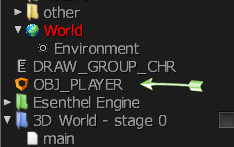
\includegraphics[width=0.4\linewidth]{../images/objClass1.png}
\caption[]{Een Object Class.}
\label{fig:objClass1}
\end{figure}

\begin{figure}[h]
\centering
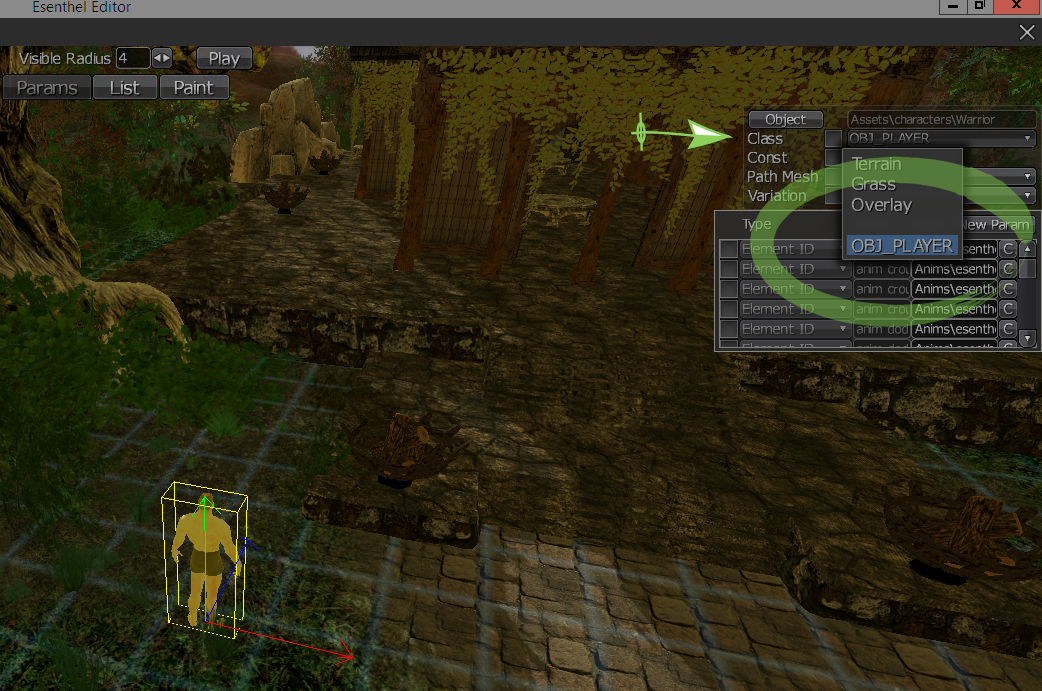
\includegraphics[width=0.9\linewidth]{../images/objClass2.png}
\caption[]{Een Object Class Toewijzen.}
\label{fig:objClass2}
\end{figure}

\begin{exercise}
Voer stap 3 en 4 uit om je class te linken aan het player object.
\end{exercise}

\subsection{Camera}
Ook voor de camera maken we een afzonderlijke class. Voorlopig heeft die enkel een update functie nodig, maar dat kan later meer worden. Je kan er van uit gaan dat je maar \'e\'en camera nodig hebt. Daarom voorzie je onder de class ook een object.

\begin{code}
class gameCam
{
	void update() 
	{
	
	}
}
gameCam GameCam;
\end{code}

Binnen de functie update bepaal je de positie van de camera en de kijkrichting. Meestal zal de camera op de player gericht zijn. Maar het kan voorkomen dat er tijdelijk geen player object bestaat, bijvoorbeeld bij het einde van het spel, of tijdens een teleport. Daarom starten we de update functie met de mogelijkheid dat er geen speler bestaat. In dat geval voeren we de camera code uit de vorige sectie uit, zodat de camera kan bewegen via de muis.

\begin{code}
if(!Players.elms())
{
	 if(Ms.b(1)) {
			Cam.transformByMouse(0.1, 100, CAMH_ZOOM | CAMH_MOVE);
	 } else
	 {
			Cam.transformByMouse(0.1, 100, CAMH_ZOOM | CAMH_ROT);
	 }
	 return;
}
\end{code}

Vervolgens update je de afstand van de camera tot zijn target. Dat doen we via de beweging van het muiswiel:

\begin{code}
Cam.dist -= Ms.wheel() * Time.d() * 10;
Clamp(Cam.dist, 2, 5);
\end{code}

En tot slot stel je de positie, yaw, pitch en target distance in:

\begin{code}
Cam.setSpherical(Players[0].ctrl.center() + Vec(0, 0.5, 0), Players[0].angle.x, Players[0].angle.y, 0, Cam.dist);
Cam.updateVelocities().set();
\end{code}

\begin{exercise}
\begin{enumerate}
	\item Werk de class gameCam uit, zoals hierboven. Vergeet niet dat je de \eeFunc{update()} functie ook moet toevoegen aan de main \eeFunc{Update()} functie.
	\item Pas enkele waarden in de camera update aan. Voer telkens je programma uit om te zien wat het resultaat is.
	\item Pass de avatar controle in \eeClass{Player.update()} aan aan je wensen. Hoe wil je je avatar besturen?
	\item Voeg aan de main \eeFunc{Update()} functie ook de volgende regels toe:
	
	\begin{code}
	D.grassUpdate();
  Water.update(Vec2(0.01, 0.01));
	\end{code}
	
	Wat is het resultaat?
\end{enumerate}
\end{exercise}











